\documentclass{ximera}

\title{Worksheets}
\author{Bart Snapp}

\begin{document}
\begin{abstract}
  We discuss the set up for a collection of worksheets.
\end{abstract}
\maketitle

%\section{Worksheets}

A worksheet is a piece of paper with questions on it. A Ximera worksheet is no
different.

\paragraph{File structure}

\begin{center}
  \scalebox{.6}{
    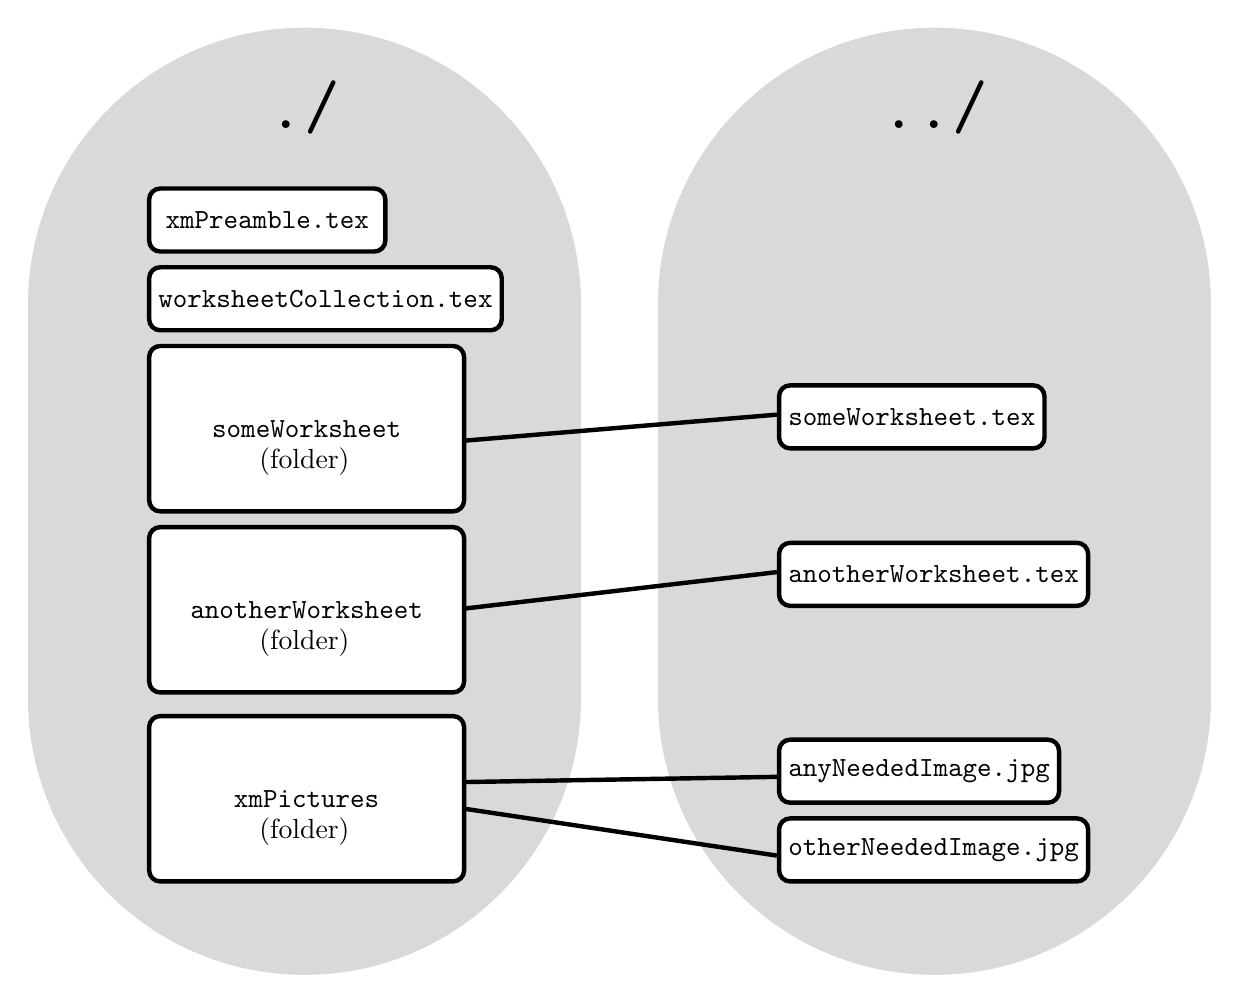
\begin{tikzpicture}
      % Define styles for nodes
      \tikzstyle{document} = [anchor=north west,draw, rounded corners,
      rectangle,
      minimum width=3cm,fill=white, minimum height=.8cm, ultra
      thick,font=\ttfamily]
      \tikzstyle{folder} = [anchor=north west,draw, rectangle, rounded corners,
      minimum width=4cm,fill=white, minimum height=2.1cm, ultra
      thick,font=\ttfamily]

      % Thick grey lines
      \draw[line width=200pt,white!85!black,line cap=round] (2,1.5) -- (2,-3.5);
      \draw[line width=200pt,white!85!black,line cap=round] (10,1.5) --
      (10,-3.5);



      % Connections
      \draw[ultra thick] (2,-.4) -- (8,.1);
      \draw[ultra thick] (2,-2.6) -- (8,-1.9);
      \draw[ultra thick] (2,-4.6) -- (8,-4.5);
      \draw[ultra thick] (2,-4.6) -- (8,-5.5);

      % Symbols at top
      \node at (2,4) {\Huge \tt ./};
      \node at (10,4) {\Huge \tt ../};

      \node[document] at (0,3) {xmPreamble.tex};
      \node[document] at (0,2) {worksheetCollection.tex};
      % Define the folders at top level
      \node[folder] at (0,1) {someWorksheet};
      \node[] at (2,-.5) {(folder)};
      \node[folder] at (0,-1.3) {anotherWorksheet};
      \node[] at (2,-2.8) {(folder)};
      \node[folder] at (0,-3.7) {xmPictures};
      \node[] at (2,-5.2) {(folder)};

      % Define the documents in the worksheets folder
      \node[document] at (8,.5) {someWorksheet.tex};
      \node[document] at (8,-4) {anyNeededImage.jpg};
      \node[document] at (8,-1.5) {anotherWorksheet.tex};
      \node[document] at (8,-5) {otherNeededImage.jpg};
    \end{tikzpicture}
  }
\end{center}

In this setting, the file \verb!worksheetCollection.tex! might look something
like
\begin{verbatim}
\document{xourse}
\author{Ada Lovelace}
\title{My Groovy Worksheets}
\begin{abstract}
  Some of my worksheets.
\end{abstract}
\maketitle
\begin{document}
\activity{someWorksheet/someWorksheet}
\activity{anotherWorksheet/anotherWorkSheet}
\end{document}
\end{verbatim}


\end{document}